\documentclass{beamer}
\usepackage[utf8]{inputenc}

\usetheme{Madrid}
\usecolortheme{default}
\usepackage{amsmath,amssymb,amsfonts,amsthm}
\usepackage{mathtools}
\usepackage{txfonts}
\usepackage{tkz-euclide}
\usepackage{listings}
\usepackage{adjustbox}
\usepackage{array}
\usepackage{tabularx}
\usepackage{gvv}
\usepackage{lmodern}
\usepackage{circuitikz}
\usepackage{tikz}
\usepackage{graphicx}

\setbeamertemplate{page number in head/foot}[totalframenumber]

\usepackage{tcolorbox}
\tcbuselibrary{minted,breakable,xparse,skins}



\definecolor{bg}{gray}{0.95}
\DeclareTCBListing{mintedbox}{O{}m!O{}}{%
  breakable=true,
  listing engine=minted,
  listing only,
  minted language=#2,
  minted style=default,
  minted options={%
    linenos,
    gobble=0,
    breaklines=true,
    breakafter=,,
    fontsize=\small,
    numbersep=8pt,
    #1},
  boxsep=0pt,
  left skip=0pt,
  right skip=0pt,
  left=25pt,
  right=0pt,
  top=3pt,
  bottom=3pt,
  arc=5pt,
  leftrule=0pt,
  rightrule=0pt,
  bottomrule=2pt,
  toprule=2pt,
  colback=bg,
  colframe=orange!70,
  enhanced,
  overlay={%
    \begin{tcbclipinterior}
    \fill[orange!20!white] (frame.south west) rectangle ([xshift=20pt]frame.north west);
    \end{tcbclipinterior}},
  #3,
}
\lstset{
    language=C,
    basicstyle=\ttfamily\small,
    keywordstyle=\color{blue},
    stringstyle=\color{orange},
    commentstyle=\color{green!60!black},
    numbers=left,
    numberstyle=\tiny\color{gray},
    breaklines=true,
    showstringspaces=false,
}
%------------------------------------------------------------
%This block of code defines the information to appear in the
%Title page
\title %optional
{2.7.8}
\date{August 25,2025}
%\subtitle{A short story}

\author % (optional)
{Harsha-EE25BTECH11026}



\begin{document}


\frame{\titlepage}
\begin{frame}{Question}
Find $|\vec{a}-\vec{b}|$, if two vectors $\vec{a}$ and $\vec{b}$ are such that $|\vec{a}|=2$,$|\vec{b}|=3$ and $\vec{a}.\vec{b}=4$.
\end{frame}



\begin{frame}{Theoretical Solution}
According to the question,\\
\begin{align}
    |\vec{a}|=2 \;\; ; \; |\vec{b}|=3 \;\; ;\; \vec{a}^T\vec{b}=4
\end{align}
\end{frame}

\begin{frame}{Equation}
The  value of $\|\vec{a}-\vec{b}\|$ can be computed by the following formula,
\begin{align}
    \|\vec{a}-\vec{b}\|^2=\|\vec{a}\|^2+\|\vec{b}\|^2-2\vec{a}^T\vec{b}
\end{align}
\end{frame}

\begin{frame}{Theoretical Solution}
\begin{align}
    \therefore \|\vec{a}-\vec{b}\|^2=2^2+3^2-2\times4
\end{align}
\begin{align}
    \|\vec{a}-\vec{b}\|^2=5
\end{align}
\begin{align}
    \implies \|\vec{a}-\vec{b}\|=\sqrt{5}=2.2361 units
\end{align}

\end{frame}



\begin{frame}[fragile]
    \frametitle{C Code - Cross product and magnitude of vector}

    \begin{lstlisting}
#include<stdio.h>

double find_mag_diffvector(double a, double b ,double dot)
//Here dot is the dot product of a and b
{
	double val=a*a+b*b-2*dot;
	if(val<0) val=0;
	return sqrt(val);
}
    \end{lstlisting}
\end{frame}



\begin{frame}[fragile]
    \frametitle{Python+C Code}
    \begin{lstlisting}
import ctypes

lib = ctypes.CDLL('./libdiff.so')

lib.find_mag_diffvector.argtypes = [ctypes.c_double, ctypes.c_double, ctypes.c_double]
lib.find_mag_diffvector.restype = ctypes.c_double

a = 2.0
b = 3.0
dot = 4.0

diff = lib.find_mag_diffvector(a, b, dot)
print(f"The magnitude of difference vector of a and b is: {diff:.4f}")

    \end{lstlisting}
\end{frame}

\begin{frame}[fragile]
    \frametitle{Python+C Code}
    \begin{lstlisting}
#taking an example of vectors a and b to prove computationally
A=(2.0,0)
B=(0,3.0)

# Plotting
plt.figure()
plt.quiver(0, 0, A[0], A[1], angles='xy', scale_units='xy', scale=1, color='r', label='a')
plt.quiver(0, 0, B[0], B[1], angles='xy', scale_units='xy', scale=1, color='b', label='b')
plt.quiver(B[0], B[1], A[0]-B[0], A[1]-B[1],
           angles='xy', scale_units='xy', scale=1, color='g', label='a-b')



    \end{lstlisting}
\end{frame}

\begin{frame}[fragile]
    \frametitle{Python+C Code}
    \begin{lstlisting}
#Annotate magnitudes
plt.text((A[0]+B[0])/2, (A[1]+B[1])/2, f"|a-b|={diff:.4f}", color='g', fontsize=10, ha='center', va='bottom')

plt.xlim(-1, 5)
plt.ylim(-1, 5)
plt.gca().set_aspect('equal', adjustable='box')
plt.grid()
plt.legend()
plt.title("Magnitude of vector difference: a - b")
plt.savefig("/home/user/Matrix/Matgeo_assignments/2.7.8/figs/Figure_1.png")
plt.show()



    \end{lstlisting}
\end{frame}




\begin{frame}[fragile]
    \frametitle{Python Code}
    \begin{lstlisting}
import math as m
import matplotlib as mp
mp.use("TkAgg")
import matplotlib.pyplot as plt
a=2.0
b=3.0
dot=4.0

def find_mag_diffvector(a,b,dot):
    diff=m.sqrt(a**2+b**2-2*dot)
    return diff

mag_diff=find_mag_diffvector(a,b,dot)

print(f"The magnitude of difference of vector a and b is :{mag_diff:.4f}")
    \end{lstlisting}
\end{frame}

\begin{frame}[fragile]
    \frametitle{Python Code}
    \begin{lstlisting}
#taking an example of vectors a and b to prove computationally
A=(2.0,0)
B=(0,3.0)

# Plotting
plt.figure()
plt.quiver(0, 0, A[0], A[1], angles='xy', scale_units='xy', scale=1, color='r', label='a')
plt.quiver(0, 0, B[0], B[1], angles='xy', scale_units='xy', scale=1, color='b', label='b')
plt.quiver(B[0], B[1], A[0]-B[0], A[1]-B[1],
           angles='xy', scale_units='xy', scale=1, color='g', label='a-b')



    \end{lstlisting}
\end{frame}

\begin{frame}[fragile]
    \frametitle{Python Code}
    \begin{lstlisting}
#Annotate magnitudes
plt.text((A[0]+B[0])/2, (A[1]+B[1])/2, f"|a-b|={diff:.4f}", color='g', fontsize=10, ha='center', va='bottom')

plt.xlim(-1, 5)
plt.ylim(-1, 5)
plt.gca().set_aspect('equal', adjustable='box')
plt.grid()
plt.legend()
plt.title("Magnitude of vector difference: a - b")
plt.savefig("/home/user/Matrix/Matgeo_assignments/2.7.8/figs/Figure_1.png")
plt.show()
    \end{lstlisting}
\end{frame}

\begin{frame}{Plot}
    \centering
    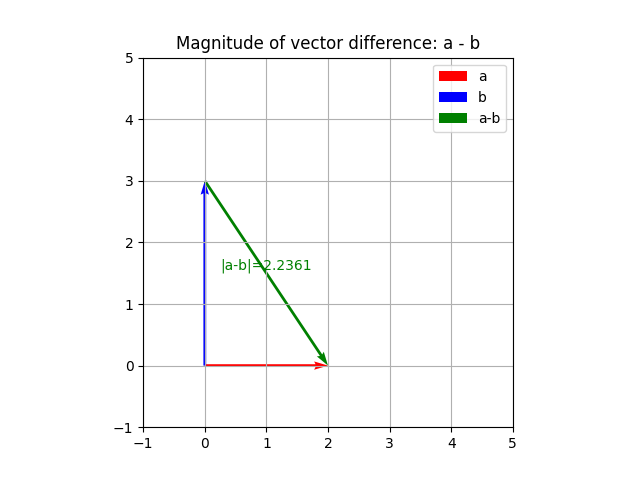
\includegraphics[width=\columnwidth, height=0.8\textheight, keepaspectratio]{figs/Figure_1.png}     
\end{frame}




\end{document}